\subsection{Обзор предметной области}


\par
Классификация текстов --- невероятно популярная задача. Мы пользуемся текстовыми классификаторами в почтовом клиенте: он классифицирует письма и фильтрует спам. Другие приложения включают классификацию документов, обзоров и так далее.

\bigskip\par
Обычно классификация текстов используется не как самостоятельная задача, а является частью более крупного пайплайна. Например, голосовой помощник классифицирует ваше высказывание, чтобы понять, что вы хотите или чувствуете и передать ваше сообщение другой модели в зависимости от решения классификатора.  Другой пример --- поисковый движок: он может использовать классификаторы для определения языка запроса, или предсказать его тип (например, развлекательный, информационный, навигационный, транзакционный) и понять хотите ли вы увидеть картинки или видео помимо документов или подобрать контент по настроению.

% \bigskip\par
% Поскольку большинство датасетов для классификации содержат только одну правильную метку. А у нас многоклассовая классификация.
\bigskip
Задачи интеллектуальной обработки текста делятся на три типа: синтаксические, основанные на понимании смысла и третий --- не просто понимание написанного, а еще и генерация нового текста. Сентимент-анализ относится ко второму типу.

\bigskip\par
Сентимент-анализ, как направление компьютерной лингвистики, стал очень популярен последние десятилетие. С
появлением больших данных насыщенных эмоциональной составляющей возникла потребность в их обработке. Компании
начали устраивать соревнования с внушительными призовыми фондами, а исследователи искать лучшую архитектуру
для классификации этих данных. Так в открытом доступе появились большие размеченные датасететы с отзывами,
данными из соцсетей и новостями.

\bigskip\par
Сам термин <<сентимент>> означает совокупность чувств и взглядов, как основа для действия или суждения; общая
эмоциональная установка. Целью сентимент-анализа является выделении этих тональных компонент из текста.
Рассмотрим его применение на разных уровнях \cite{Semina}.

\bigskip\par
Пусть есть целый документ, тогда, как правило, в нем можно выделить один субъект и один объект, а так же
сентимент. Ярким примером такого уровня является отзыв. Здесь автор выступает в качестве субъекта, а предмет
отзыва --- в качестве объекта. Это уровень документа.

\bigskip\par
Если документ более сложный, то можно рассматривать его на уровне предложений. В результате можно определить
эмоциональную окраску всего документа или предложений по отдельности. Зависит от поставленной задачи.

\bigskip\par
Также анализ бывает на уровне аспектов. Смысл его в том, что эмоциональная установка определяется не для
конкретно объекта, а для его отдельных составляющих --- аспектов. Например, для объекта <<компьютер>> можно
выделить аспекты <<производительность>>, <<дизайн>>, <<сборка>> т.д., другими словами, к аспектам относится
все то, к чему могут быть выражены эмоции. Данная задача очень востребована, потому что позволяет точнее
определять отношение автора к объекту, а для некоторых задач это очень важный критерий.

\bigskip\par
Последний вид анализа самый сложный и проводится уровне именованных сущностей (Named Entities). Именованная
сущность --- это абстрактный или физический объект, который может быть обозначен собственным именем. Сама по
себе задача извлечения именованных сущностей (Named Entity Recognition) не из простых, а вкупе с
сентимент-анализом становится действительно комплексным решением.

% https://habr.com/ru/company/mailru/blog/516214/
% https://ieeexplore.ieee.org/document/9117010/references#references

\bigskip\par
Методы сентимент анализа можно также разделить на несколько основных направлений \cite{Semina}:
\bigskip
\begin{itemize}
 \item \textit{метод основанный на правилах (rule-based).} Здесь используются наборы правил классификации, составленные экспертом и эмоционально размеченные словари. Определенный класс присваивается в зависимости от найденных ключевых слов и их использования с другими ключевыми словами. Такой метод достаточно эффективный, но
 очень трудоемкий. Неплохих результатов в бинарной классификации добились в работе \cite{atex};

 \item \textit{метод основанный на словарях.} Самый простой метод, основанный  на подсчете сентиментных единиц содержащихся в словарях тональности. Очень сильно зависит от размера словаря и не очень точен в разрыве с правилами русского языка. Попытка получения сентимента из текста таким способом описана в этой работe \cite{Kirill};

 \item \textit{методы основанные на машинном и глубоком обучении.} (machine learning, deep learning) Наиболее популярная группа методов в сентимент-анализе, работающих на способности алгоритмов обобщать выделенные из текста признаки. Их применение позволило получить очень высокие результаты в работах \cite{senti1, senti2, senti3, senti4};

 \item \textit{гибридные методы.} Позволяют одновременно использовать несколько подходов. % ++ дописать сюжа
что-нибудь
\end{itemize}

\bigskip\par
Разберем подробнее машинное и глубокое обучение. Суть метода в выделении признаков из текста и последующем их
обобщении с помощью разнообразных алгоритмов. Для выделения признаков используют, как простые алгоритмы по
типу мешок слов (Bag of Words) или TF-IDF, так и небольшие нейронные сети для генерирования эмбеддингов,
например, Word2Vec \cite{Mikolov:1}, GloVe \cite{glove}, FastText \cite{fasttext}. Существуют и более сложные алгоритмы, которые формируют признаки на уровне предложений, к ним относятся ELMo \cite{elmo1,elmo2}, BERT (Bidirectional Encoder Representations from Transformers) \cite{bert} и др.

\bigskip\par
Чтобы обработать выделенные признаки используют разнообразные алгоритмы. К классическому обучению относятся:

\bigskip
\begin{itemize}
 \item байессовский классификатор (Naive Bayes classifier);
 \item дерево решений (Decision Tree);
 \item логистическая регрессия (Logistic Regression);
 \item метод опорных векторов (Support Vector Machine).
\end{itemize}

\bigskip\par
Среди алгоритмов глубокого обучения можно выделить:
\begin{itemize}
 \item реккурентные нейронные сети (RNN);
 \item сверточные нейронные сети (CNN);
 \item полносвязные нейронные сети (FCNN) и т.д.
\end{itemize}


\subsection{Задача классификации и сентимент-анализа текстов}

\noindent
Что такое естественный язык вообще, и как с ним работают?

\bigskip
\begin{itemize}
 \item множество допустимых цепочек символов из некоторого алфавита;
 \item цепочки строятся по некоторым правилам;
 \item текст --- одна такая цепочка
 \item алфавит --- множество символов, из которых строятся тексты языка
 \item далеко не каждая цепочка несет какую-то информацию
\end{itemize}

\bigskip\noindent
Анализ языка сводится к двум глобальным задачам:

\bigskip
\begin{itemize}
 \item обучение: понять правила языка;
 \item применение: для некоторого текста понять по каким правилам он построен.
\end{itemize}

\bigskip
В этой работе задача классификации сформулирована следующим образом. Пусть есть описание документа $d \in X$, где $X$ --- векторное пространство документов и фиксированный набор меток $C = \{c_1, c_2, \ldots, c_n\}$. Из обучающей выборки (множества документов с заранее известными метками --- эмоциями) $D = \{\langle d, c \rangle | \langle d, c \rangle\ \in X \times C\}$ и с помощью метода обучения $G$ необходимо получить классифицирующую функцию $G(D) = f$, которая отображает документы в пространство меток $f : X \to C$.


\subsection{Предобработка текстов}

Представим, что у нас есть набор данных с текстами на русском языке и соответствующие им метки. Для автоматической обработки текста в рассматриваемой задаче удобно было бы представить слова в начальной форме. Для этого применяется лемматизация текста.

\begin{definition}
 Лемматизация --- процесс приведения словоформы к лемме --- нормальной (словарной) форме.
\end{definition}

\bigskip
\fbox{Квартира простояла пустой и запечатанной только неделю.} $\to$ \fbox{квартира простаивать пустой и запечатывать только неделя}

\bigskip
Как правило текст хорошо описывает словарь из которого состоит набор данных, и тем как часто они встречаются в тексте, а не структурой фразы. Проведем небольшой эксперимент: возьмем набор данных, который рассматривается в этой работе, посчитаем для каждого слова в этом наборе частоту его встречаемости и отсортируем полученный список по убыванию частот. Получили график распределения Ципфа рис. \ref{fig:ciph} --- распределения вероятностей, описывающего взаимоотношения частоты события и количества событий с такой частотой.

\begin{figure}[ht]
    \centering
    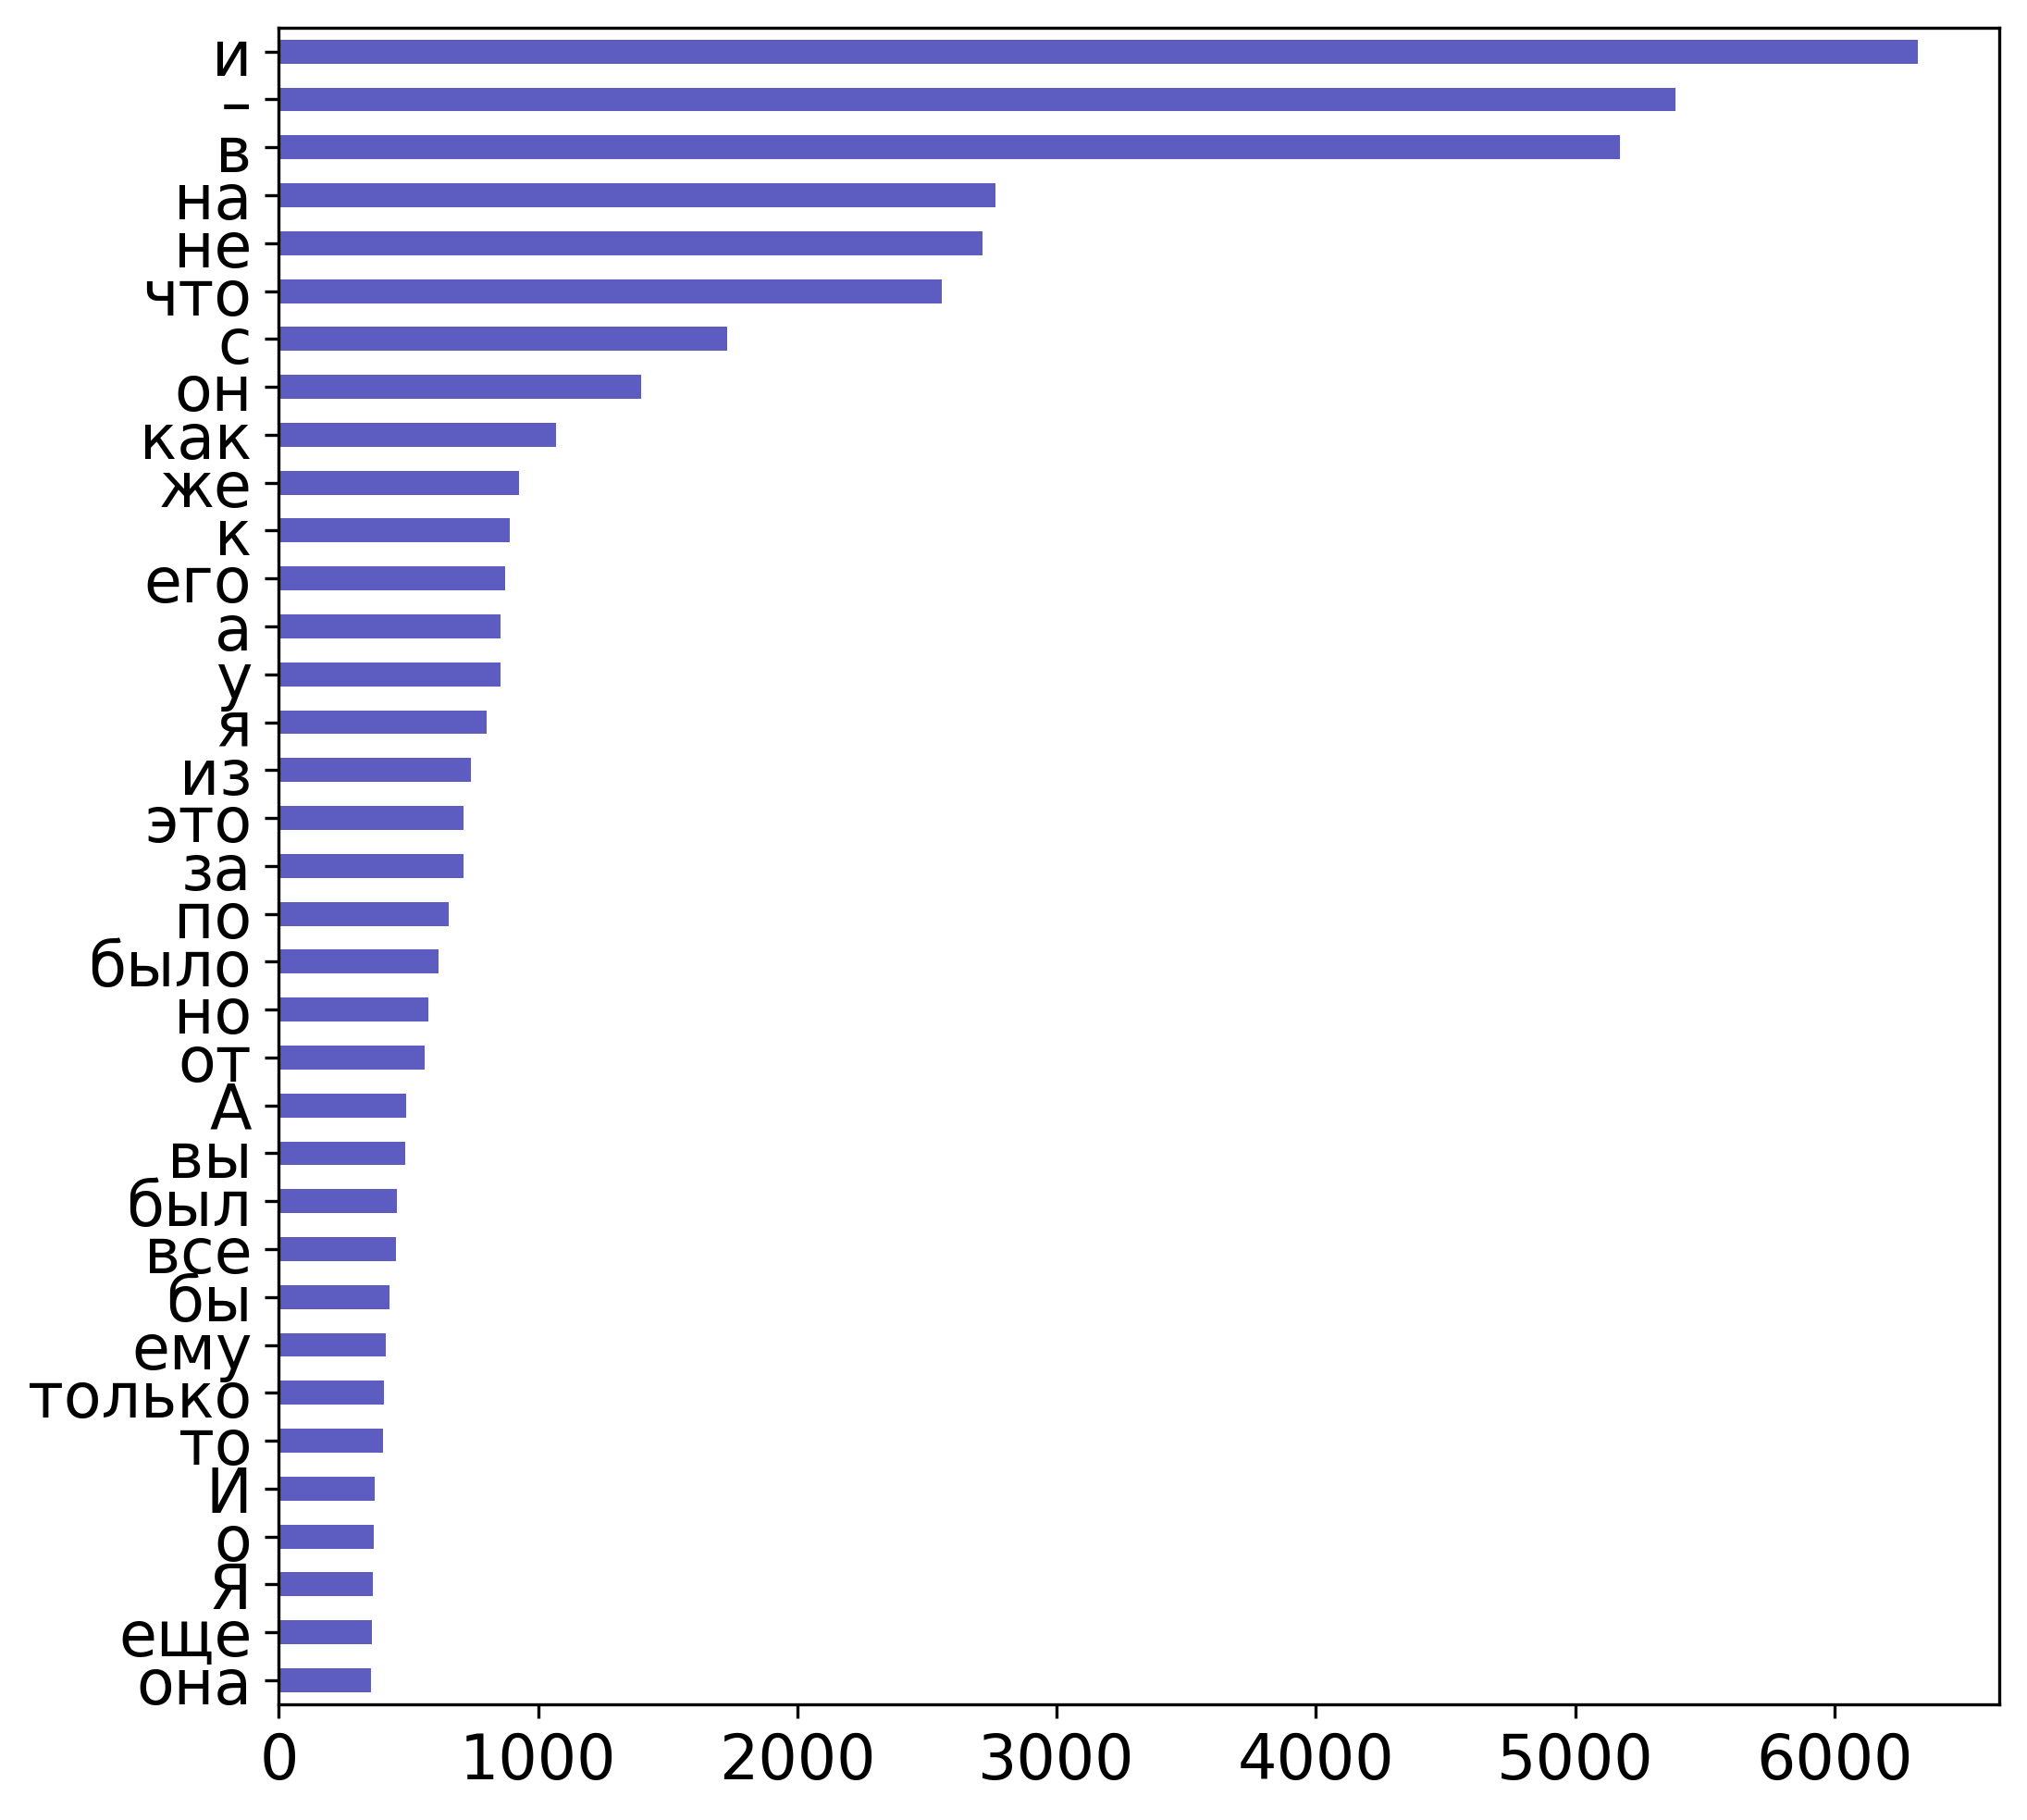
\includegraphics[scale=0.5]{ciph.png}
    \caption{График частоты встречаемости слов и символов в наборе данных}
    \label{fig:ciph}
\end{figure}

\bigskip\noindent
Это распределение представляет собой степенную функцию:

\begin{equation*}
 f(rank:s,N) = \frac{1}{Z(s,N)rank^s},
\end{equation*}

\bigskip
где $rank$ --- порядковый номер слова после сортировки по убыванию частоты, $s$ --- коэффициент скорости убывания вероятности, $N$ --- количество слов и $Z(s,N)= \sum_(i=1)^N i^{-s}$ --- нормализованная константа.

\bigskip\noindent
Из этого графика можно сделать три основных вывода:

\bigskip
\begin{itemize}
 \item частотных слов мало и они не информативны;
 \item редких слов много, они информативны, но на них сложно опираться;
 \item нужен баланс частотности и информативности.
\end{itemize}

\bigskip
Самые частотные и не значимые слова называются <<стоп-словами>>. Для русского языка определены словари стоп-слов, программная реализация есть в библиотеке <<nltk>>. Обработка предыдущего предложения дает такой результат:

\bigskip
\fbox{квартира простаивать пустой и запечатывать только неделя} $\to$ \fbox{квартира простаивать пустой запечатывать неделя}

\bigskip\noindent
На рис. \ref{fig:ciph_lem} представлено  распределение частотности слов после лемматизации и удаления стоп-слов.

\begin{figure}[ht]
    \centering
    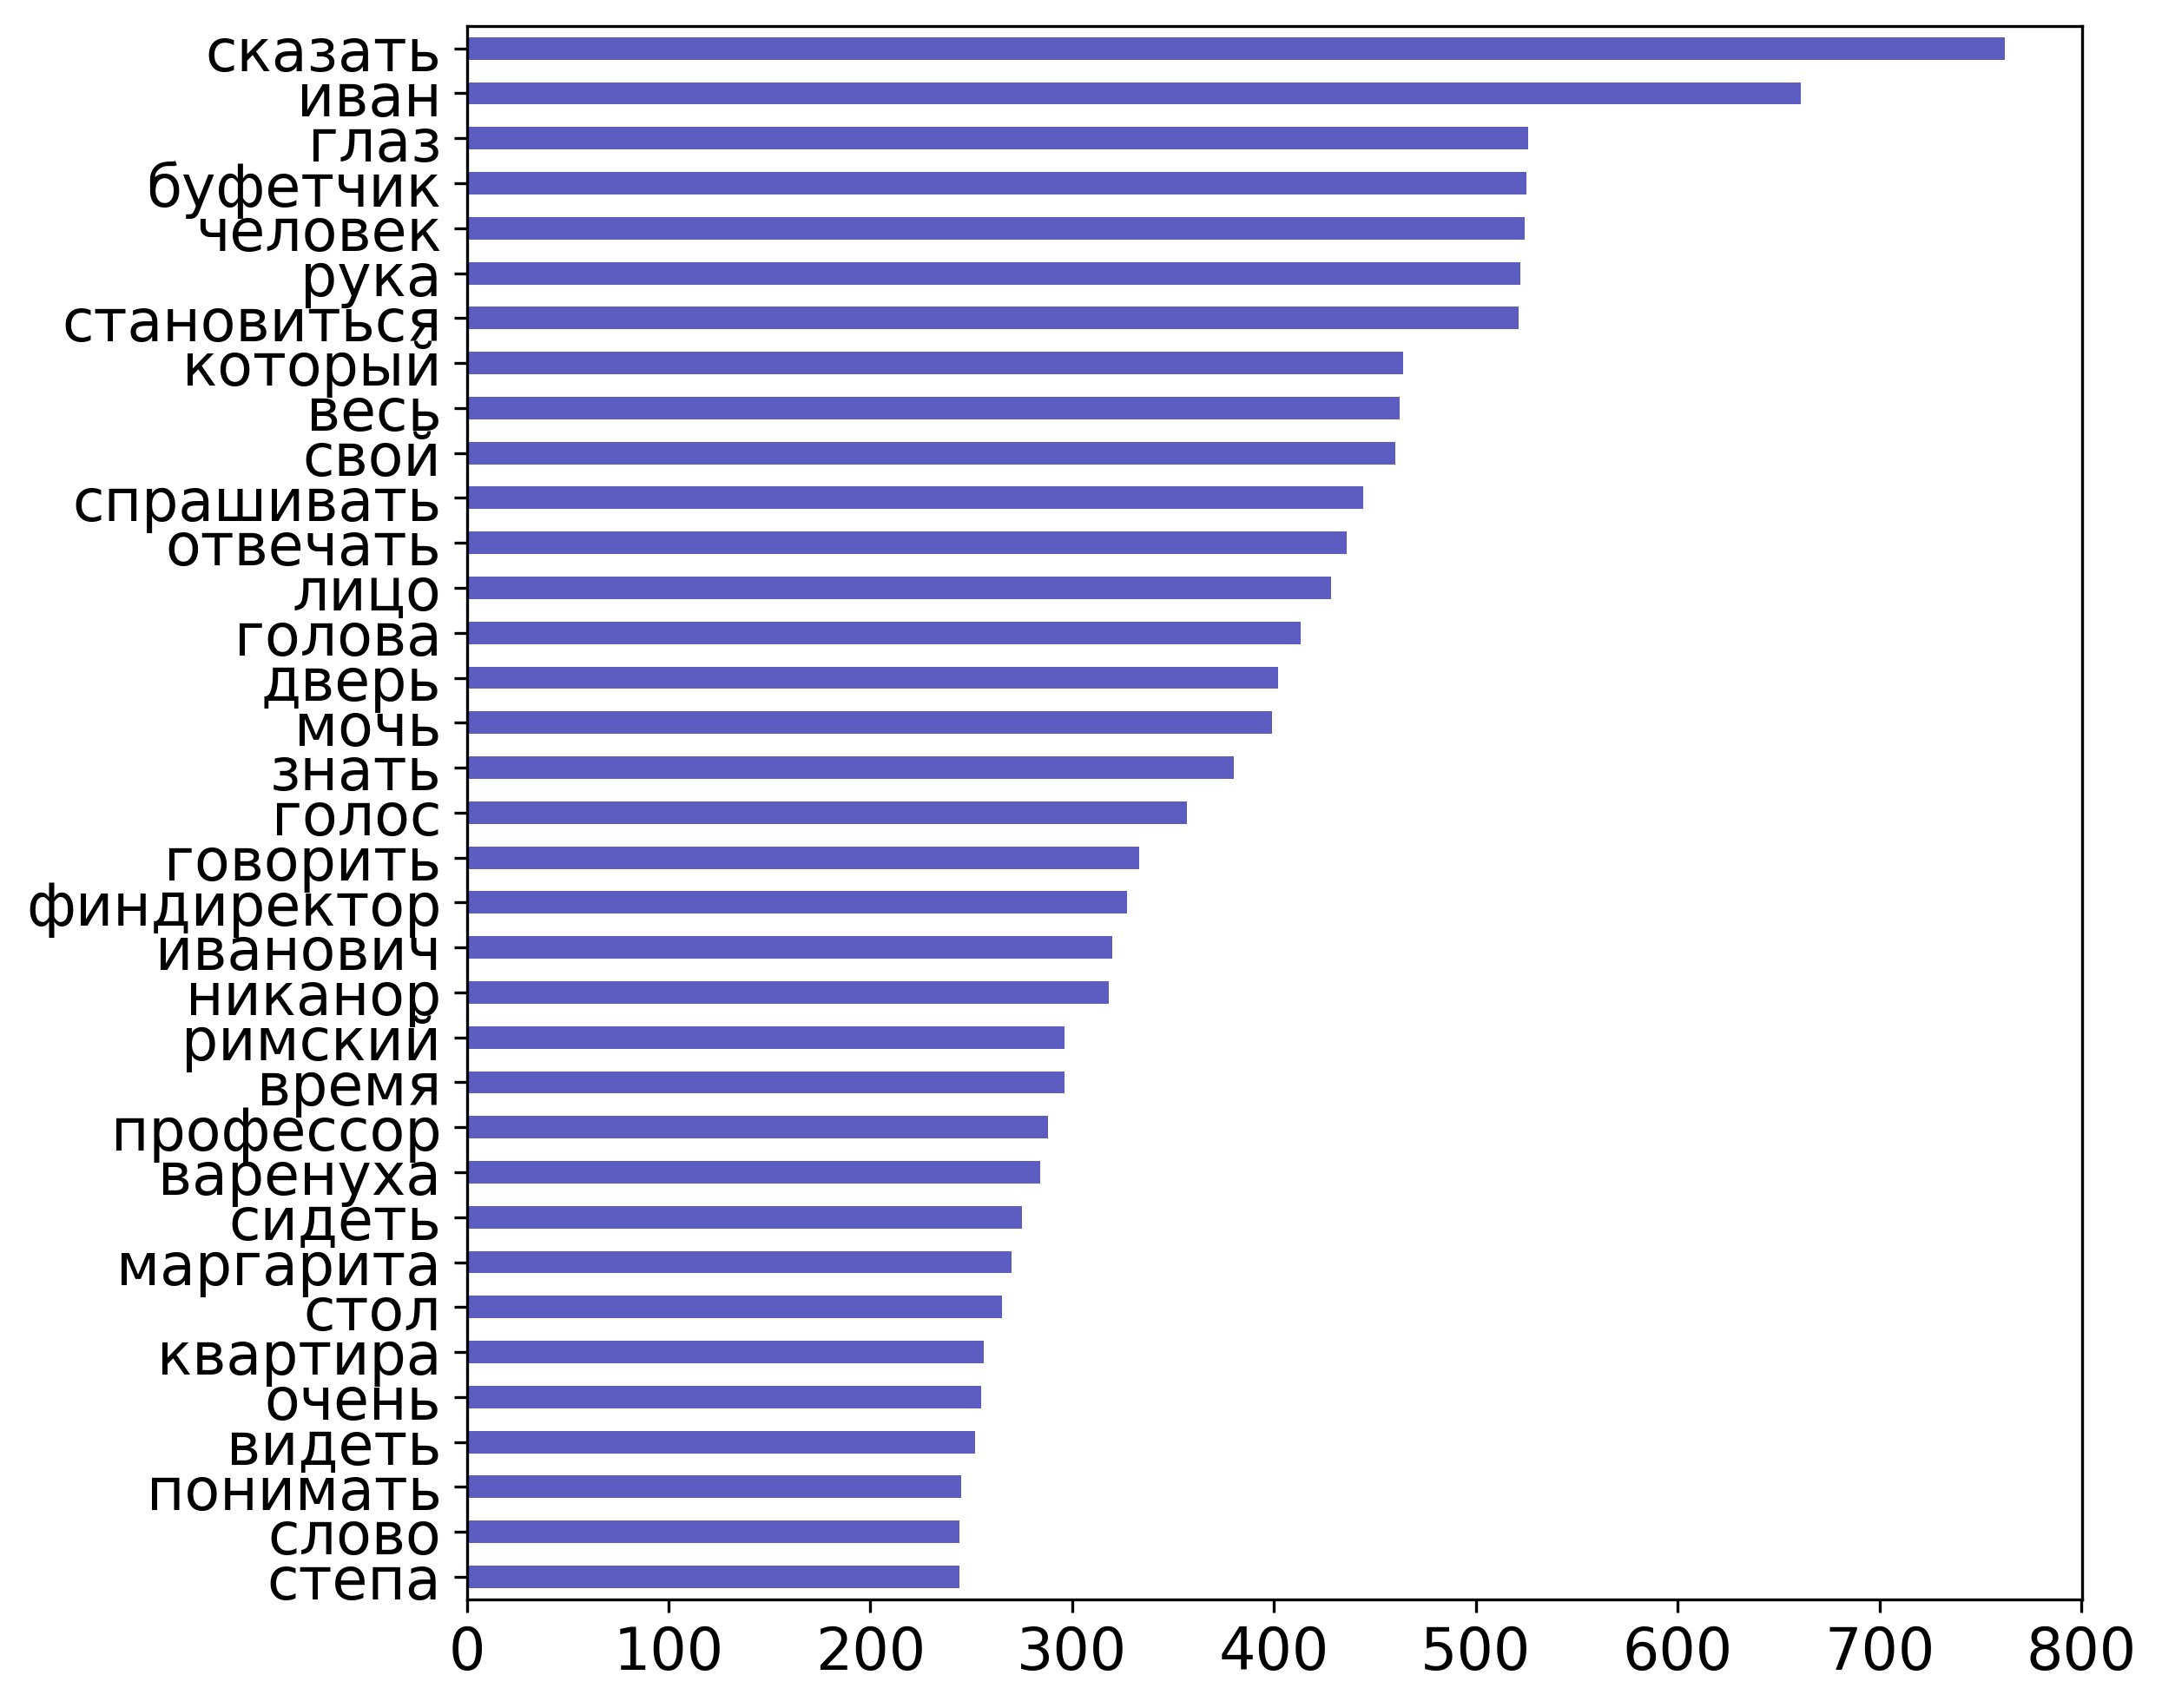
\includegraphics[scale=0.5]{ciph_lem.png}
    \caption{График частоты встречаемости слов в наборе данных после обработки}
    \label{fig:ciph_lem}
\end{figure}



